% !TEX root = ./busty_transcription.tex
\section{Finding the ``right'' model: Bayesian parameter inference and model selection}
\subsection{Parameter inference for constitutive promoters}

From consideration of Fano factors in the previous section, we suspect that
model 5 in~\fig{fig:constit_cartoons}, a one-state bursty model of constitutive
promoters, achieves a Goldilocks level of complexity. Does this stand up to
closer scrutiny, namely, comparison to full mRNA distributions rather than
simply their moments? We will test this thoroughly on all the data from
constitutive promoters from Jones et.\ al.~\cite{Jones2014}.

It will be instructive, however, to first consider the Poisson promoter, model 1
in~\fig{fig:constit_cartoons}. As we alluded to earlier, since the Poisson
distribution has its Fano factor $\nu$ strictly equal to 1,
and all of the observed data has Fano factor $\nu>1$, we might
already suspect that this model is incapable of fitting the data.
We will verify that this in fact the case. As a consequence
of ruling out model 1, models 2 and 3 will also be ruled out.
Why? Again all the data have $\nu>1$, meaning the mRNA distributions
are overdisperse compared with a Poisson distribution,
while models 2 and 3 have Fano factors $\nu\le 1$ meaning they
are underdisperse relative to Poisson. So models 2 and 3
can fare no better than the simple Poisson model. We will also not explicitly
consider model 4 from~\fig{fig:constit_cartoons} since it was already thoroughly
analyzed in~\cite{Razo-Mejia2020}, and since model 5 can be viewed as a special
case of it.

In performing parameter inference on the FISH data of~\cite{Jones2014}, building
a generative model is straightforward. The data are single-cell mRNA counts, and
we assume different cells to be independent and identically distributed from the
underlying generative model, which is just the steady-state mRNA distribution
computed from the master equation of the underlying model.

\subsubsection{Model 1: Poisson promoter}
\mmnote{A lot of the details I've written here might be excessive for main text and serve better as an intro-by-example to Bayes in the appendix, then reduce main text to a bit more bare bones?}
For this model the master equation of interest is~\eq{eq:poisson_promoter_cme}
with repressor set to zero, i.e.,
\begin{equation}
\deriv{t}p_{m,U}(t) = rp_{m-1,U}(t) - rp_{m,U}(t)
        + (m+1)\gamma p_{m+1,U}(t) - \gamma p_{m,U}(t),
\end{equation}
whose steady-state distribution is Poisson, given by
\begin{equation}
p_U(m) = \frac{\lambda^m e^{-\lambda}}{m!}
\end{equation}
with $\lambda=r/\gamma$. This steady state distribution defines our likelihood
$p(m\mid\lambda)$, i.e.
\begin{equation}
p(m\mid\lambda) = \frac{\lambda^m e^{-\lambda}}{m!}
\label{eq:poisson_inference010}
\end{equation}
is the probability of observing a single cell with $m$ mRNAs given a known value
of $\lambda$, written to make the conditioning explicit.

With our likelihood in hand, we can invoke Bayes theorem to write down the
posterior distribution on our model parameter $\lambda$, given by
\begin{equation}
p(\lambda\mid D) \propto p(D\mid\lambda) p(\lambda),
\end{equation}
where our data $D=\{m_1, m_2,\dots, m_N\}$ is a list of mRNA counts over a
population of $N$ identical cells. As is standard we have neglected the factor
$p(D)$ on the right hand side since it is independent of $\lambda$ and serves
only as a normalization factor. Since we assume each cell's mRNA count is
independent of others, the likelihood is simply a product of the single cell
likelihoods given by \eq{eq:poisson_inference010} above, so
\begin{equation}
p(D\mid\lambda) = \prod_{k=1}^N \frac{\lambda^{m_k}e^{-\lambda}}{m_k!}.
\end{equation}
This is often notated simply as
\begin{equation}
D \sim \text{Poisson}(\lambda),
\end{equation}
which is read as the data $D$ is Poisson
distributed with mean $\lambda$. The $\sim$ operator literally denotes ``is
distributed according to.''
The conditioning on $\lambda$ is no longer explictily notated,
only implied by its appearance on the right hand side.

To proceed we need to specify a prior. In this case we are extremely data-rich,
as the dataset from Jones et.\ al~\cite{Jones2014} has of order 1000-3000
single-cell measurements for each promoter, so our choice of prior matters
little here, as long as it does not exclude the true value of $\lambda$. A
convenient choice for our problem is to use a \textit{conjugate} prior.
A conjugate prior is a special prior that causes the posterior to
have the same functional form as the prior, simply with updated
model parameters. This makes calculations
analytically tractable and also offers a nice interpretation of the inference
procedure as updating our knowledge about the model parameters.
This makes conjugate priors very useful when they exist.
The caveat is that conjugate priors only exist for a very limited
number of likelihoods, mostly with only one or two model
parameters, so in almost all other Bayesian inference problems,
we must tackle the posterior numerically.

But, for the problem at hand, a conjugate prior does in fact exist.
For a Poisson likelihood of identical and identically distributed
data, the conjugate prior is a gamma distribution, as
can be looked up in, e.g.,~\cite{Gelman2013}, Section 2.6.
Putting a gamma prior on $\lambda$ introduces two new parameters $\alpha$ and
$\beta$ which parametrize the gamma distribution itself, which we use to encode
the range of $\lambda$ values we view as reasonable. Recall $\lambda$ is the
mean steady-state mRNA count per cell, which \textit{a priori} could plausibly
be anywhere from 0 to a few hundred. $\alpha=1$ and $\beta=1/50$ achieve this,
since the gamma distribution is strictly positive with mean $\alpha/\beta$ and
standard deviation $\sqrt{\alpha}/\beta$. To be explicit, then, our prior is
\begin{equation}
\lambda \sim \text{Gamma}(\alpha, \beta)
\end{equation}

As an aside, note that if we did not know that our prior was a conjugate prior,
we could still write down our posterior distribution from its definition as
\begin{equation}
p(\lambda\mid D,\alpha,\beta)
\propto p(D\mid\lambda) p(\lambda \mid\alpha,\beta)
\propto \left(\prod_{k=1}^N \frac{\lambda^{m_k}e^{-\lambda}}{m_k!}\right)
        \frac{\beta}{\Gamma(\alpha)}(\beta\lambda)^{\alpha-1} e^{-\beta\lambda}
.
\end{equation}
Without foreknowledge that this in fact reduces to a gamma distribution, this
expression might appear rather inscrutable. When conjugate priors are
unavailable for the likelihood of interest - which is almost always the case for
models with $>1$ model parameter - this inscrutability is the norm, and making
sense of posteriors analytically is almost always impossible. Fortunately, MCMC
sampling provides us a powerful method of constructing posteriors numerically
which we will make use of extensively.

Since we did use a conjugate prior, we may simply look up our posterior in any
standard reference such as~\cite{Gelman2013}, Section 2.6,
from which we find that
\begin{equation}
\lambda
\sim \text{Gamma}\left(\alpha + \bar{m}N, \beta + N\right),
\end{equation}
where we defined the sample mean $\bar{m} = \frac{1}{N}\sum_k m_k$ for
notational convenience. A glance at the FISH data from~\cite{Jones2014} reveals
that $N$ is $\mathcal{O}(10^3)$ and $\langle m\rangle \gtrsim 0.1$ for all
constitutive strains in~\cite{Jones2014}, so $\bar{m}N \gtrsim 10^2$. Therefore
as we suspected, our prior parameters are completely overwhelmed by the data.
The prior behaves, in a sense, like $\beta$ extra ``data points''
with a mean value of $(\alpha-1)/\beta$~\cite{Gelman2013}, which
gives us some intuition for how much data is needed to overwhelm
the prior in this case: enough data $N$ such that $\beta\ll N$
and $\alpha/\beta \ll \bar{m}$. In
fact, $\bar{m}N$ and $N$ are so large that we can, to an excellent
approximation, ignore the $\alpha$ and $\beta$ dependence and approximate the
gamma distribution as a Gaussian with mean $\bar{m}$ and standard deviation
$\sqrt{\bar{m}/N}$, giving
\begin{equation}
\lambda
\sim \text{Gamma}\left(\alpha + \bar{m}N, \beta + N\right)
\approx \text{Normal}\left(\bar{m}, \sqrt{\frac{\bar{m}}{N}}\right).
\end{equation}
As an example with real numbers, for the \textit{lacUV5} promoter, Jones et.\
al~\cite{Jones2014} measured 2648 cells with an average mRNA count per cell of
$\bar{m} \approx 18.7$. In this case then, our posterior is
\begin{equation}
\lambda
\sim \text{Normal}\left(18.7, 0.08\right),
\end{equation}
which suggests we have inferred our model's one parameter to a precision of
order 1\%.

This is not wrong, but it is not the full story. The model's posterior is
tightly constrained, but is it a good generative model? In other words, does the
model generate data that look similar to our actual data, and is it therefore
plausible that the model captures the important features of the data generating
process? This intuitive notion can be codified with \textit{posterior predictive
checks}, or PPCs, and we will see that this simple Poisson model fails badly.

The intuitive idea of posterior predictive checks is simple: \mmnote{Not sure if
all this stuff is clearer by example, but then does it confuse the reader in
generalizing to other models?}
\begin{enumerate}
\item Make a random draw of the model parameter $\lambda$ from the posterior
distribution.
\item Plug that draw into the likelihood and generate a synthetic dataset
$\{m_k\}$ conditioned on $\lambda$.
\item Repeat many times.
\end{enumerate}
More formally, the posterior predictive distribution can be thought of as the
distribution of future yet-to-be-observed data, conditioned on the data we have
already observed. Clearly if those data appear quite different, the model has a
problem. Put another way, if we suppose the generative model is true, then the
synthetic datasets we generate should resemble the actual observed data, and if
not, it suggests the model is missing important features. All the data we
consider in this work are 1D (distributions of mRNA counts over a population) so
ECDFs are an excellent visual means of comparing synthetic and observed
datasets. In general for higher dimensional datasets, much of the challenge is
in merely designing good visualizations that can actually show if synthetic and
observed data are similar or not.

For our example Poisson promoter model then, we merely draw many random numbers,
say 1000, from the Gaussian posterior. For each one of those draws, we generate
a dataset from the likelihood, i.e., we draw 2648 (the number of observed cells
in the actual dataset) Poisson-distributed numbers for each of the 1000
posterior draws, for a total of 2648000 samples from the posterior predictive
distribution.

To compare so many samples with the actual observed data, one excellent
visualization for 1D data is ECDFs of the quantiles, as shown for our Poisson
model in~\fig{fig:constit_post_full}.
In this example, the median for each possible mRNA
count is shown as a dark green line, while shaded bands of lighter
green contain 95\% of the posterior predictive samples.
Plotting quantiles in this way gives us a sense of the range of data we might
consider plausible, under the assumption that the model is true. In this case it
is quite obvious that the observed data, plotted in orange, could not plausibly
come from this Poisson generative model. The other model with a PPC plotted
in~\fig{fig:constit_post_full}, bursty model 5 with
a negative binomial steady-state mRNA
distribution, looks like a good candidate by eye. We cover it in more detail
later.

\subsubsection{Nonequilibrium Model Five - Bursty promoter}
Let us now consider the problem of parameter inference from FISH data
for model five from~\fig{fig1:means_cartoons}(C). As derived
in Appendix~\ref{sec:gen_fcn_appdx}, the steady-state mRNA distribution
in this model is a negative binomial distribution,
given by~\eq{eq:nbinom_deriv_final}, which is
\begin{equation}
p(m) = \frac{\Gamma(m+k_i)}{\Gamma(m+1)\Gamma(k_i)}
        \left(\frac{1}{1+b}\right)^{k_i}
        \left(\frac{b}{1+b}\right)^m,
\end{equation}
where $b$ is the mean burst size and $k_i$ is the burst rate
nondimensionalized by the mRNA degradation rate $\gamma$.
As sketched earlier, the story of this distribution is of
geometrically-distributed bursts of mRNA, where the arrival of bursts is a
Poisson process with rate $k_i$ and the mean size of a burst is $b$.

As for the Poisson promoter model, this expression for the steady-state
mRNA distribution is exactly the likelihood we want to use in Bayes theorem.
Again denoting the single-cell mRNA count data as $D=\{m_1, m_2,\dots, m_N\}$,
here Bayes theorem takes the form
\begin{equation}
p(k_i, b \mid D) \propto p(D\mid k_i,b)p(k_i, b).
\end{equation}
We already have our likelihood so we only need to choose priors
on $k_i$ and $b$. For the datasets from~\cite{Jones2014} that we
are analyzing, as for the Poisson promoter model above we are
still data-rich so the prior's influence remains weak, but not
nearly as weak because the dimensionality of our model has
increased from one to two.

We follow the guidance of~\cite{Gelman2013}, Section 2.9 in
opting for weakly-informative priors on $k_i$ and $b$ (conjugate
priors do not exist for this problem), and we find
``street-fighting estimates''~\cite{Mahajan2010} to be an ideal
way of constructing such priors. The idea of weakly informative
priors is to allow all remotely plausible values of model
parameters while excluding the completely absurd or unphysical.

Consider $k_i$. The fastest known bacterial promoters control
rRNA genes and initiate transcripts no faster than $\sim
1/\text{sec}$. It would be exceedingly strange if any of the
constitutive promoters from~\cite{Jones2014} were stronger than
that, so we can take that as an upper bound. For a lower bound,
if transcripts are produced too rarely, there would be nothing to
see with FISH. The datasets for each strain contain of order
$10^3$ cells, and if the $\langle m \rangle = k_i b/\gamma
\lesssim 10^{-2}$, then the total number of expected mRNA
detections would be single-digits or less and we would have
essentially no data on which to carry out inference. So assuming
$b$ is not too different from 1, justified next, and an mRNA
lifetime of $\gamma^{-1}\sim 3-5~\text{min}$, this gives us soft
bounds on $k_i/\gamma$ of perhaps $10^{-2}$ and $3\times 10^1$.

Next consider mean burst size $b$. This parametrization of the
geometric distribution allows bursts of size zero (which could
representing aborted transcripts and initiations), but it would
be quite strange for the mean burst size $b$ to be below
$\sim10^{-1}$, for which nearly all bursts would be of size zero
or one. For an upper bound, if transcripts are initiating at a
rate somewhat slower than rRNA promoters, then it would probably
take a time comparable to the lifetime of an mRNA to produce a
burst larger than 10-20 transcripts, which would invalidate the
approximation of the model that the duration of bursts are
instantaneous compared to other timescales in the problem. So we
will take soft bounds of $10^{-1}$ and $10^1$ for $b$.

Note that the natural scale for these ``street-fighting estimates''
was a log scale. This is commonly the case that our prior sense
of reasonable and unreasonable parameters is set on a log scale.
A natural way to enforce these soft bounds is therefore to use a
lognormal prior distribution, with the soft bounds set $\pm2$
standard deviations from the mean.

With this, we are ready to write our full generative model as
\begin{equation}
\begin{split}
\ln k_i \sim \text{Normal}(-0.5, 2)
\\
\ln b \sim \text{Normal}(0.5, 1)
\\
m \sim \text{NBinom}(k_i, b).
\end{split}
\end{equation}
We carried out MCMC sampling on the posterior of this model, starting
with the constitutive \textit{lacUV5} dataset from~\cite{Jones2014}.
The resulting MCMC samples are shown in~\fig{fig:constit_post_full}(A).
In constrast to the active/inactive constitutive model considered
in~\cite{Razo-Mejia2020} (nonequilibrium model four
in~\ref{fig:constit_cartoons}), this model is well-identified
with both parameters determined to a fractional uncertainty of 5-10\%.
The strong correlation reflects the fact that their product sets
the mean of the mRNA distribution, which is tightly constrained
by the data, but there is weak ``sloppiness''~\cite{Transtrum2015}
along a set of values with a similar product.

Flush with success having found the model's posterior to be
well-identified, the next step was posterior predictive sampling.
The only procedural difference compared to the Poisson promoter
model is that, since we have no analytical posterior expression
but only samples from the posterior, we generate a synthetic
dataset (i.e., posterior predictive samples) for each posterior
sample from the MCMC sampling. \fig{fig:constit_post_full}(B)
shows the resulting predictive ECDF; similarly to the Poisson
promoter model, the median posterior predictive ECDF is plotted
as a dark blue line, while a lighter blue shaded region
encompasses 95\% of the posterior predictive samples. Unlike the
Poisson promoter model, the experimental ECDF closely tracks the
posterior predictive ECDF, indicating this model is actually able
to generate the observed data and increasing our confidence that
this model is at least not wrong.

\textit{lacUV5} is our primary target here, since it forms the
core of all the simple repression constructs of~\cite{Jones2014}
that we consider in Section~\ref{sec:rep_kinetics_inference}.
Nevertheless, we thought it wise to apply our bursty promoter
model to the other 17 constitutive promoters available in the
FISH dataset from~\cite{Jones2014} as a test that the model is
capturing the essential phenomenology. If the model fit well to
all the different promoters, this would increase our confidence
that it would serve well as a foundation for inferring repressor
kinetics later in Section~\ref{sec:rep_kinetics_inference}.
Conversely, were the model to fail on more than a couple of the
other promoters, it would give us pause.

\begin{figure}%[h!]
\centering
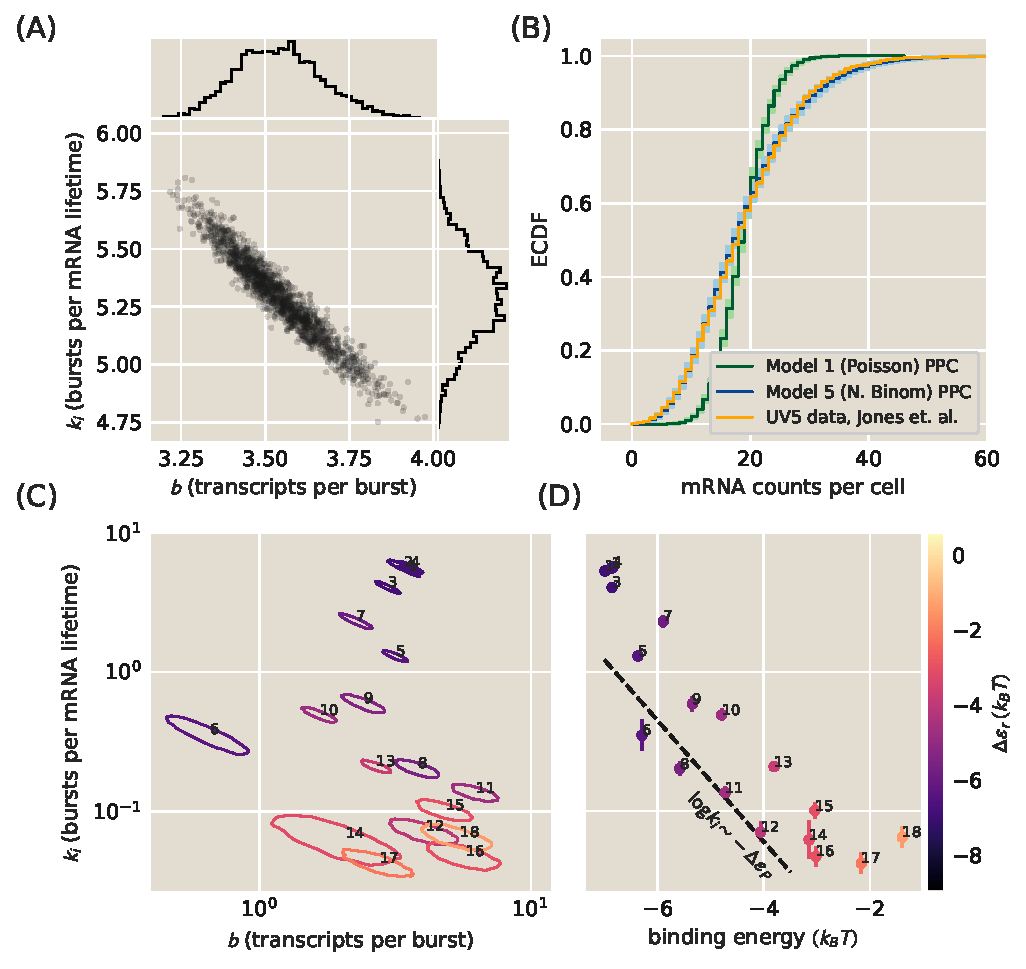
\includegraphics[width=\textwidth]{../figures/main/fig03.pdf}
\caption{\textbf{Constitutive promoter posterior inference and model
        comparison.}
        (A) The joint posterior density of model 5, the
        bursty promoter with negative binomially-distributed
        steady state, is plotted with MCMC samples.
        1D marginal densities are plotted as flanking histograms.
        The model was fit on \textit{lacUV5} data from~\cite{Jones2014}.
        (B) The ECDF of the observed population distribution of
        mRNA transcripts under the control of a constitutive
        lacUV5 promoter is shown in orange.
        The median posterior predictive ECDFs for models (1),
        Poisson, and (5), negative binomial, are plotted in
        green and blue, respectively.
        Lighter green and blue regions enclose 95\% of all
        posterior predictive samples from their respective models.
        Model (1) is in obvious contradiction with the data
        while model (5) is not.
        FISH data is again from~\cite{Jones2014}.
    (C) Joint posterior distributions for burst rate $k_i$ and mean burst size
    $b$ for 18 promoters from~\cite{Jones2014}. Each contour indicates the 95\%
    highest posterior density region for a particular promoter. Note that the
    vertical axis is shared with (D). Panel (D) plots the burst rate $k_i$ vs.\
    the binding energy for each promoter from energy matrices
    from~\cite{Brewster2012}.
    The dotted line shows the predicted slope according to
    $\ln k_i/\gamma \sim \text{constant} - \beta\Delta\epsilon_P$,
    described in text.}
\label{fig:constit_post_full}
\end{figure}

\fig{fig:constit_post_full}(C) shows the results, plotting the
posterior distribution from individually MCMC sampling all 18
constitutive promoter datasets from~\cite{Jones2014}. To aid
visualization, rather than plotting samples for each promoter's
posterior as we did in \fig{fig:constit_post_full}(A), for each
posterior we find and plot the curve that surrounds the 95\%
highest probability density region, i.e., on a plot analogous
to~(A), each contour would enclose approximately 95\% of the
samples, and thus 95\% of the probability mass,
of its posterior distribution.
Posterior predictive ECDFs (not shown) display a similar level of
agreement between data and predictive samples as for the bursty
model with \textit{lacUV5} in \fig{fig:constit_post_full}(B).
\mmnote{Might be worth showing some/all of these PPCs in
supplement for completeness? We could do postage stamp sized diff
plots and probably fit all 18 promoters on 1-2 pages.}

One interesting feature from \fig{fig:constit_post_full}(C) is
that burst rate varies far more widely, over a range of
$\sim10^2$, than burst size, confined to a range of
$\lesssim10^1$ (and with the exception of promoter 6, just a span
of 3-5x). This suggests that $k_i$, not $b$, is the key dynamic
variable that promoter binding site tunes.

It is interesting to connect this observation to the work
of~\cite{Brewster2012}, where these same 18 promoters were
considered through the lens of the three-state equilibrium model
and binding energies $\Delta\epsilon_P$ were predicted from an
energy matrix model derived from~\cite{Kinney2010}. The connection
is made simply by equating mean mRNA levels in both theories,
\mmnote{derivation is hasty, needs elaboration}
\begin{equation}
\langle m \rangle = \frac{k_i b}{\gamma}
        = \frac{r}{\gamma}
        \frac{\frac{P}{N_{NS}}\exp(-\beta\Delta\epsilon_P)}
                {1+\frac{P}{N_{NS}}\exp(-\beta\Delta\epsilon_P)},
\end{equation}
and taking the weak-promoter limit in the equilibrium model,
\begin{equation}
\langle m \rangle = \frac{k_i b}{\gamma}
        = \frac{r}{\gamma} \frac{P}{N_{NS}}\exp(-\beta\Delta\epsilon_P),
\end{equation}
valid for all the binding energies considered here.

How are the two coarse-grainings related? The only association that makes dimensional sense and produces the correct order-of-magnitude for the known parameters is to take
\begin{equation}
\frac{k_i}{\gamma} = \exp(-\beta\Delta\epsilon_P)
\label{eq:bursty_equil_corresp1}
\end{equation}
and
\begin{equation}
b = \frac{r}{\gamma}\frac{P}{N_{NS}}.
\label{eq:bursty_equil_corresp2}
\end{equation}
\fig{fig:constit_post_full}(D) shows that this linear scaling
between $\ln k_i$ and $-\beta\Delta\epsilon_P$ is approximately
true for all 18 constitutive promoters considered. The intercept
is an uninteresting function of the unknown model parameters, so
we only consider the slope of the scaling in
\fig{fig:constit_post_full}(D).
\mmnote{Wait, is that true or can we do something with the intercept, related to the burst size in some useful way? Needs more careful thought.}

While the associations represented by
\eq{eq:bursty_equil_corresp1} and \eq{eq:bursty_equil_corresp2}
appear to be born out by the scaling $\ln k_i \sim
-\beta\Delta\epsilon_P$, we do not find the association of
parameters encoded by
\eqrange{eq:bursty_equil_corresp1}{eq:bursty_equil_corresp2}
intuitive. If some deeper insight is waiting to be gleaned from it,
we leave it as an open problem.

\mmnote{Outline, still to cover:
\begin{itemize}
\item All 18 promoters. Hey the model still works on things other than UV5,
cool. Interesting and somewhat counterintuitive scaling b/w burst rate and
binding energy. Puzzle in comparing w/ Chong2014 supercoiling model. Are we
missing important things?? Unclear, we leave as open question. Good enough for
our purposes: posterior is identifiable, PPC is great, and of the models we've
thought of it is unique in satisfying both.
\end{itemize}
}

\mmnote{Discuss puzzling comparison w/ Chong2014: if supercoiling is the thing, why are my burst sizes all the same but burst rates vary? And why is the duty cycle of my promoter so low, ie., bursts so short? COmpare their fig 7E; their $\beta/\alpha$ is my $k^+/k^-$. They have one or two genes with very small $\beta/\alpha$, does the \textit{galK} locus just happen to be that, or is there a deeper disagreement? Hard to say w/o more data.}

\subsection{Transcription factor kinetics can be inferred from FISH measurements}
\label{sec:rep_kinetics_inference}
\mmnote{Outline:
\begin{itemize}
\item Full model. Write Bayes, handwave 2F1 dist story in limits of weak,
strong, and intermediate repression.
\item Hey look it mostly works. With full model, 9D model is well identified,
though most of the individual experiments unsurprisingly are not: only the ratio
of repressor rates is identifiable. PPC is not perfect, it kinda misses some
rep/op pairs but overall it's surprisingly predictive considering how strong
were the assumptions that went into it.
\item Do we chalk this up to experimental imperfections or is there interesting
biology to be found in the disagreements? I'm inclined towards the former. Even
just catching cells in truly apples-to-apples growth phases, or matching up
parameters of imaging sessions weeks or months apart, is hardly trivial.
\item The alternative is to refine our model and/or add on complexity, and it's
not at all clear what additions to make to the model, especially how to produce
the long tail of repressed strains over UV5. I see no way to get that without
getting into complicated time-correlation/history effects, where
transcription...rebounds?? After being repressed?? Sounds odd.
\item Comparison between my inferred rates, equilibrium binding E, and
single-molecule measurements. Not quite as slam-dunk as I'd hoped because of
$\gamma$ dependence, but rates are w/in factor of 2 or better, seems quite good
really! With exception of one Oid data data point, free energies are w/in about
0.5 kT also. That's not massively larger than the repeatability threshold of
fold-change measurements, at maybe 0.1 to 0.3 kT.
\item Surprising that so many model parameters can be inferred from just a few
distributions that, by eye, don't have strong features! Does require some
assumptions, e.g., about equivalence of rates across experiments, but that seems
quite reasonable.
\end{itemize}
}

\fig{fig3:kR_inferences} presents inferred
transcription factor rates, compares them to
single-molecule measurements, and compares their ratios to gold-standard binding
energies.
\begin{figure}%[h!]
\centering
\includegraphics[width=0.9\textwidth]{../figures/fig3/fig3.ai}
\caption{\textbf{Simple repression model comparison.}
Panel (A) depicts the cartoon of simple repression for which we infer parameters.
\mmnote{Not sure panel (A) is necessary, we've already shown it in at least 2
other figs. We could instead show some alternative slices of 9D posterior as a
companion to (B), or something totally different\dots??}
(B) Contours which enclose 50\% and 95\% of the posterior
probability mass are shown for of several 2D slices of
the 9D posterior distribution, from fitting one
unbinding rate for each operator (O1, O2, O3) and one binding rate for each aTc
concentration (corresponding to an unknown mean repressor copy number). (C)
Ratios of our inferred unbinding rates are compared with operator binding energy
differences measured in Garcia \& Phillips 2011 (triangles) and Razo-Mejia et.\
al.\ 2018 (squares). (D) Unbinding rates inferred in this work are compared with
single-molecule measurements of the same from Hammar et.\ at.\ 2014
\mmnote{Johan Elf's group}. Values are of similar order of magnitude, but a
precise quantitative comparison unfortunately depends sensitively on the assumed
mRNA lifetime, which was not measured.}
\label{fig3:kR_inferences}
\end{figure}

\begin{figure}%[h!]
\centering
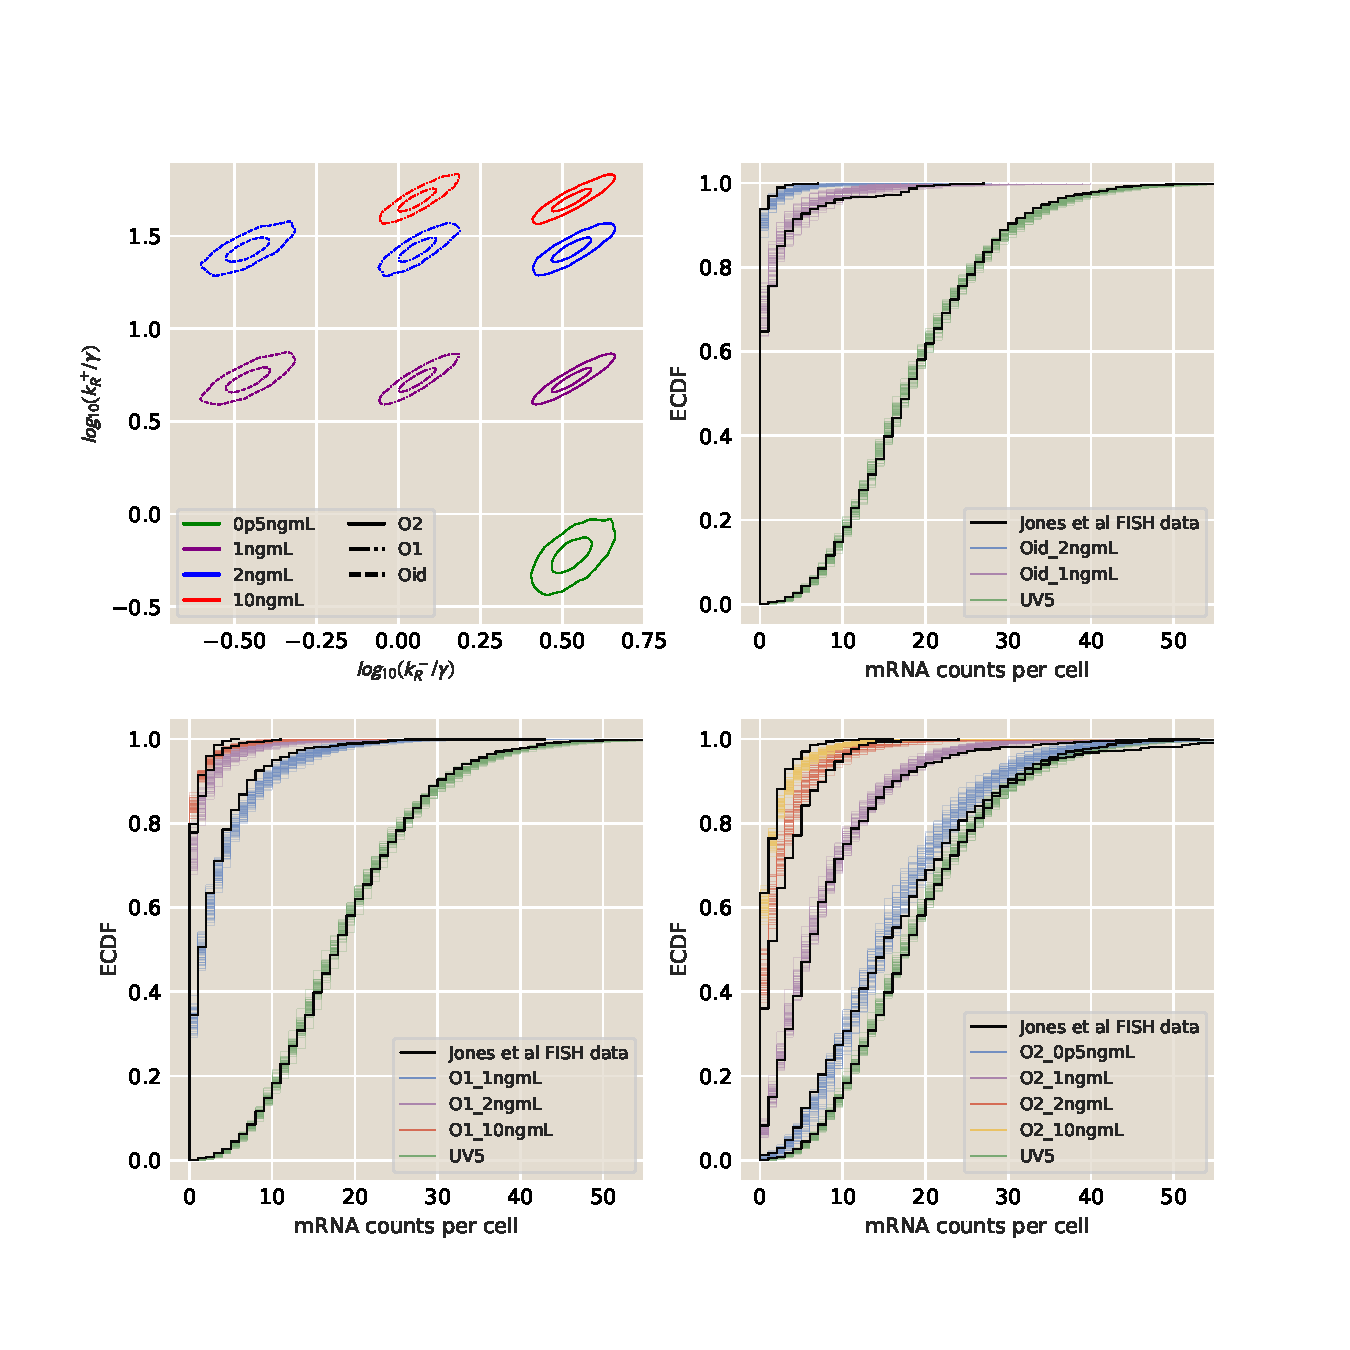
\includegraphics[width=0.9\textwidth]{../figures/figSIxx/ppc_many_pooled.pdf}
\caption{\textbf{Posterior predictive checks.}
(A) The posterior distribution from~\fig{fig3:kR_inferences}B is
shown again for context. (B), (C), and (D) Samples from the
posterior predictive distribution are shown for each of the datasets
used in the inference. Samples are sorted by operator and plotted separately
simply for visual clarity. The unrepressed promoter, UV5, is shown with each as
a reference point. \mmnote{Obviously the PPC is not perfect, but considering the
relative simplicity of the model, I'm pleasantly surprised how well it worked
and that the model was even identifiable at all. Interestingly, and perhaps not
surprisingly, only 3 of the 9 datasets were identifiable if fit in isolation:
otherwise, it was only by making assumptions that certain rates are equal across
datasets was identifiability achieved.}}
\label{fig4:ppc}
\end{figure}